%!TEX root = ../dokumentation.tex

\chapter{Einleitung}
\section{Motivation}
In der heutigen Zeit sind Fahrzeuge mit diversen Fahrerassistenzsystemen  zur Teilautomatisierung des Fahrens bereits auf dem Markt etabliert. Viele Fahrzeuge können automatisch einparken oder die Spur unter bestimmten Bedingungen halten. Der Trend bewegt sich seit Jahren von der Teilautomatisierung bestimmter Funktionen dazu immer mehr Funktionen zu automatisieren. Ein besonderer Meilenstein in dieser Entwicklung konnte bereits 2007 durch die DARPA Urban Challenge erreicht werden. Hier zeigten verschiedene Forscherteams die Machbarkeit von autonomen Fahrzeugen. Das autonome Fahren verspricht Komfortgewinn aber auch Kosteneinsparungen durch das Wegfallen von bezahlten Fahrern und erhöhte Sicherheit. Im Jahr 2018 starb laut Statistischem Bundesamt \cite{STA18} 3180 Menschen in Verkehrsunfällen. Über 300.000 Menschen wurden verletzt. Von den erfassten Unfällen lassen sich 88\% auf menschliches Fehlverhalten zurückführen.
Somit wird erwartet, dass diese Zahlen mit Durchsetzung des autonomen Fahrens drastisch zurückgehen werden. Daher forschen im Moment zahlreiche Universitäten, Fahrzeughersteller und Zulieferer an der Umsetzung des autonomen Fahren. Die Herausforderung dabei ist insbesondere der Entwurf geeigneter Softwarestrukturen und die sichere Implementierung einzelner Module für diese Systeme.

\section{Carolo-Cup Wettbewerb}
Der Carolo-Cup ist ein Hochschulwettbewerb an der Technischen Universität Braunschweig. Das Ziel des Carolo-Cups ist es, dass sich Studentierdenteams  mit der Entwicklung und Umsetzung von autonomen Modellfahrzeugen beschäftigen.

Die Modellfahrzeuge werden in unterschiedlichen realitätsnahen Szenarien miteinander verglichen und bewertet. Im Basic-Cup, der Anfängerklasse des Wettbewerbs, müssen zwei Strecken von den Modellfahrzeugen befahren werden. Eine dieser Strecken ist in Abbildung \ref{EIN:FOT} zu sehen. Im \"Obstacle Evasion\" Kurs müssen die autonomen Fahrzeuge stehende und bewegliche Hindernisse überholen. Im "Free Drive" Kurs muss das Fahrzeug möglichst viele Meter Strecke fahren. Auf beiden Strecken sollte das Fahrzeug zwei Mal autonom an einem dafür markierten Abschnitt der Strecke einparken. Zudem stellen die Teams als Teil des Wettbewerbs die erarbeiteten Konzepte einer Fachjury aus Wirtschaft und Wissenschaft vor. Dabei werden neben der Schlüssigkeit des Gesamtkonzeptes Aspekte wie Projektmanagement, Energie- und Kosteneffizienz bewertet. 
\FloatBarrier
\begin{figure}[h]
  \centering
  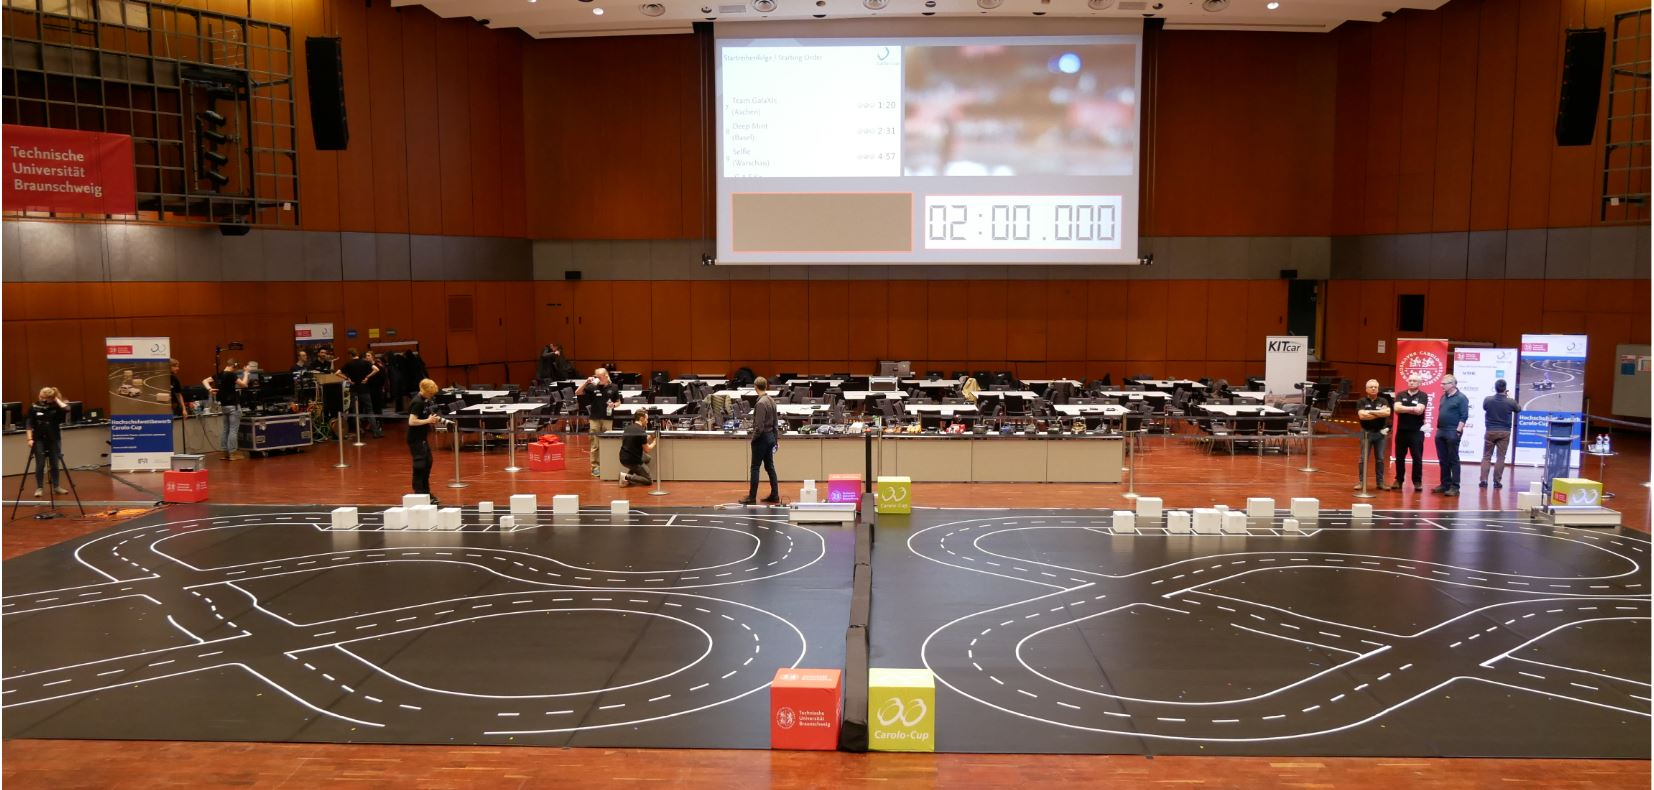
\includegraphics[width=\textwidth]{images/Einleitung/Carolocup.JPG}
  \caption[Strecke des Carolo-Cup 2020 an der TU Braunschweig]{Strecke des Carolo-Cup 2020 an der TU Braunschweig}
  \label{EIN:FOT}
\end{figure}
\FloatBarrier

\section{Zielsetzung}

Zur Zeit existieren verschiedene Ansätze, um die Software für autonome Fahrzeuge zu strukturieren. In dieser Arbeit wird eine Softwarearchitektur ausgewählt, mit der die Aufgabenstellung des Carolo-Cup 2020 erfüllt werden kann. Es wird festgelegt, wie der Datenfluss im Fahrzeug gestaltet werden soll und aus welchen Modulen das System bestehen soll. Die Architektur soll zudem möglichst leicht erweiterbar und nachvollziehbar sein.

Eine weitere wichtige Konzeptentscheidung ist die Wahl der Plattform für das autonome Fahrzeug. Es wird zwischen verschiedenen Betriebssystemen und Rechnersystemen abgewogen. Dabei wird beachtet, welche Umgebung die schnelle Erprobung neuer Softwarebestandteile erlaubt. Die Ausführung der Software soll dabei möglichst performant und unter Echtzeitbedingung erfolgen. Zudem wird die Verhaltenssteuerung des autonomen Fahrzeugs als Teil dieser Arbeit entwickelt. Dieser Teil der Software entscheidet, welches Manöver das Fahrzeug zu einem bestimmten Zeitpunkt durchführen soll. Dies kann beispielsweise die Einleitung eines Überholmanövers oder eines Parkvorgangs sein. Um Entscheidungen zu treffen, greift die Verhaltenssteuerung auf aufbereitete Sensorsignale zurück. Die Verhaltenssteuerung steuert zudem die Lichter des Fahrzeugs, um die Manöver und den Zustand des Fahrzeugs anzuzeigen. Zusätzlich soll die Verhaltenssteuerung Eingaben der Fernsteuerung und der Tasten am Fahrzeug verarbeiten. 
